\documentclass[draft,ef]{agutexSI2019}
\usepackage{graphicx}
% for table formatting
\usepackage{array}
\usepackage{booktabs} 
\usepackage{ragged2e}
\newcolumntype{P}[1]{>{\RaggedRight\arraybackslash}p{#1}}
\usepackage{makecell}
\setkeys{Gin}{draft=false}

%% ------------------------------------------------------------------------ %%
%  ENTER PREAMBLE
%% ------------------------------------------------------------------------ %%

% Author names in capital letters:
\authorrunninghead{MEEGAN-KUMAR ET AL.}

% Shorter version of title entered in capital letters:
\titlerunninghead{ESM STRUCTURE SHAPES BIASES IN SIMULATED NAM RAINFALL}

%Corresponding author mailing address and e-mail address:
\authoraddr{Corresponding author: D. Meegan-Kumar,
Department of Earth System Science, University of California Irvine,
Croul Hall 300, Irvine, CA, 92627, USA.
(dervlak@uci.edu)}

\begin{document}

%% ------------------------------------------------------------------------ %%
%  TITLE
%% ------------------------------------------------------------------------ %%
%\includegraphics{agu_pubart-white_reduced.eps}
\title{Supporting Information for ``Earth system model structure shapes biases in simulated North American monsoon rainfall"}
DOI: 10.1002/%insert paper number here%

%% ------------------------------------------------------------------------ %%
%  AUTHORS AND AFFILIATIONS
%% ------------------------------------------------------------------------ %%
\authors{Dervla Meegan-Kumar\affil{1},Jane W. Baldwin\affil{1,2}}

\affiliation{1}{Department of Earth System Science, University of California Irvine, Irvine, California}
\affiliation{2}{Lamont-Doherty Earth Observatory, Columbia University, Palisades, New York}


\begin{article}

%% ------------------------------------------------------------------------ %%
%  MAIN
%% ------------------------------------------------------------------------ %%
\noindent\textbf{Contents of this file}
\begin{enumerate}
\item Text S1
\item Figures S1 to S5
\item Table S1
\end{enumerate}

\noindent\textbf{Introduction}
This supporting information provides additional validation of the results presented in the main manuscript. This includes (1) details on the calculation of peak height underestimation following interpolation of observed topography to coarse-resolution grids (Text S1, Figure S2), (2) validation of the robustness of the HighResMIP and CM2.5-FLOR models' precipitation biases calculated against different observational and reanalysis products (Figures S1, S3), and (3) sensitivity of the computed change in future precipitation relative to the historical baseline in HighResMIP models to the time intervals used to define the future and historical baseline (Figures S4, S5).

\clearpage

\noindent\textbf{Text S1.}
Re-gridding of ETOPO05 \cite{center93ngdcn} to the idealized grids was performed with the python package xesmf with conservative remapping of area-integrated quantities (Figure \ref{fig:etopo_idealized_regrid}a--d). Then, we determined the meridional maximum elevation between 250\textdegree{E}--258\textdegree{E}, and 21\textdegree{N}--31\textdegree{N}, which covers the extent of the Sierra Madre Occidental range. For every grid-cell of the native ETOPO05 data, we determined the difference between the maximum surface height elevation of the native ETOPO05 data and the re-gridded profiles. Finally, we took the mean of those differences to represent the average elevation the re-gridded topographic data underestimates the original by.


%% ------------------------------------------------------------------------ %%
%%  REFERENCE LIST AND TEXT CITATIONS
\bibliography{high-res_hitopo_nam} 

\end{article}
\clearpage


%% ------------------------------------------------------------------------ %%
%%  FIGURES

\begin{figure}[ht]
    \centering
    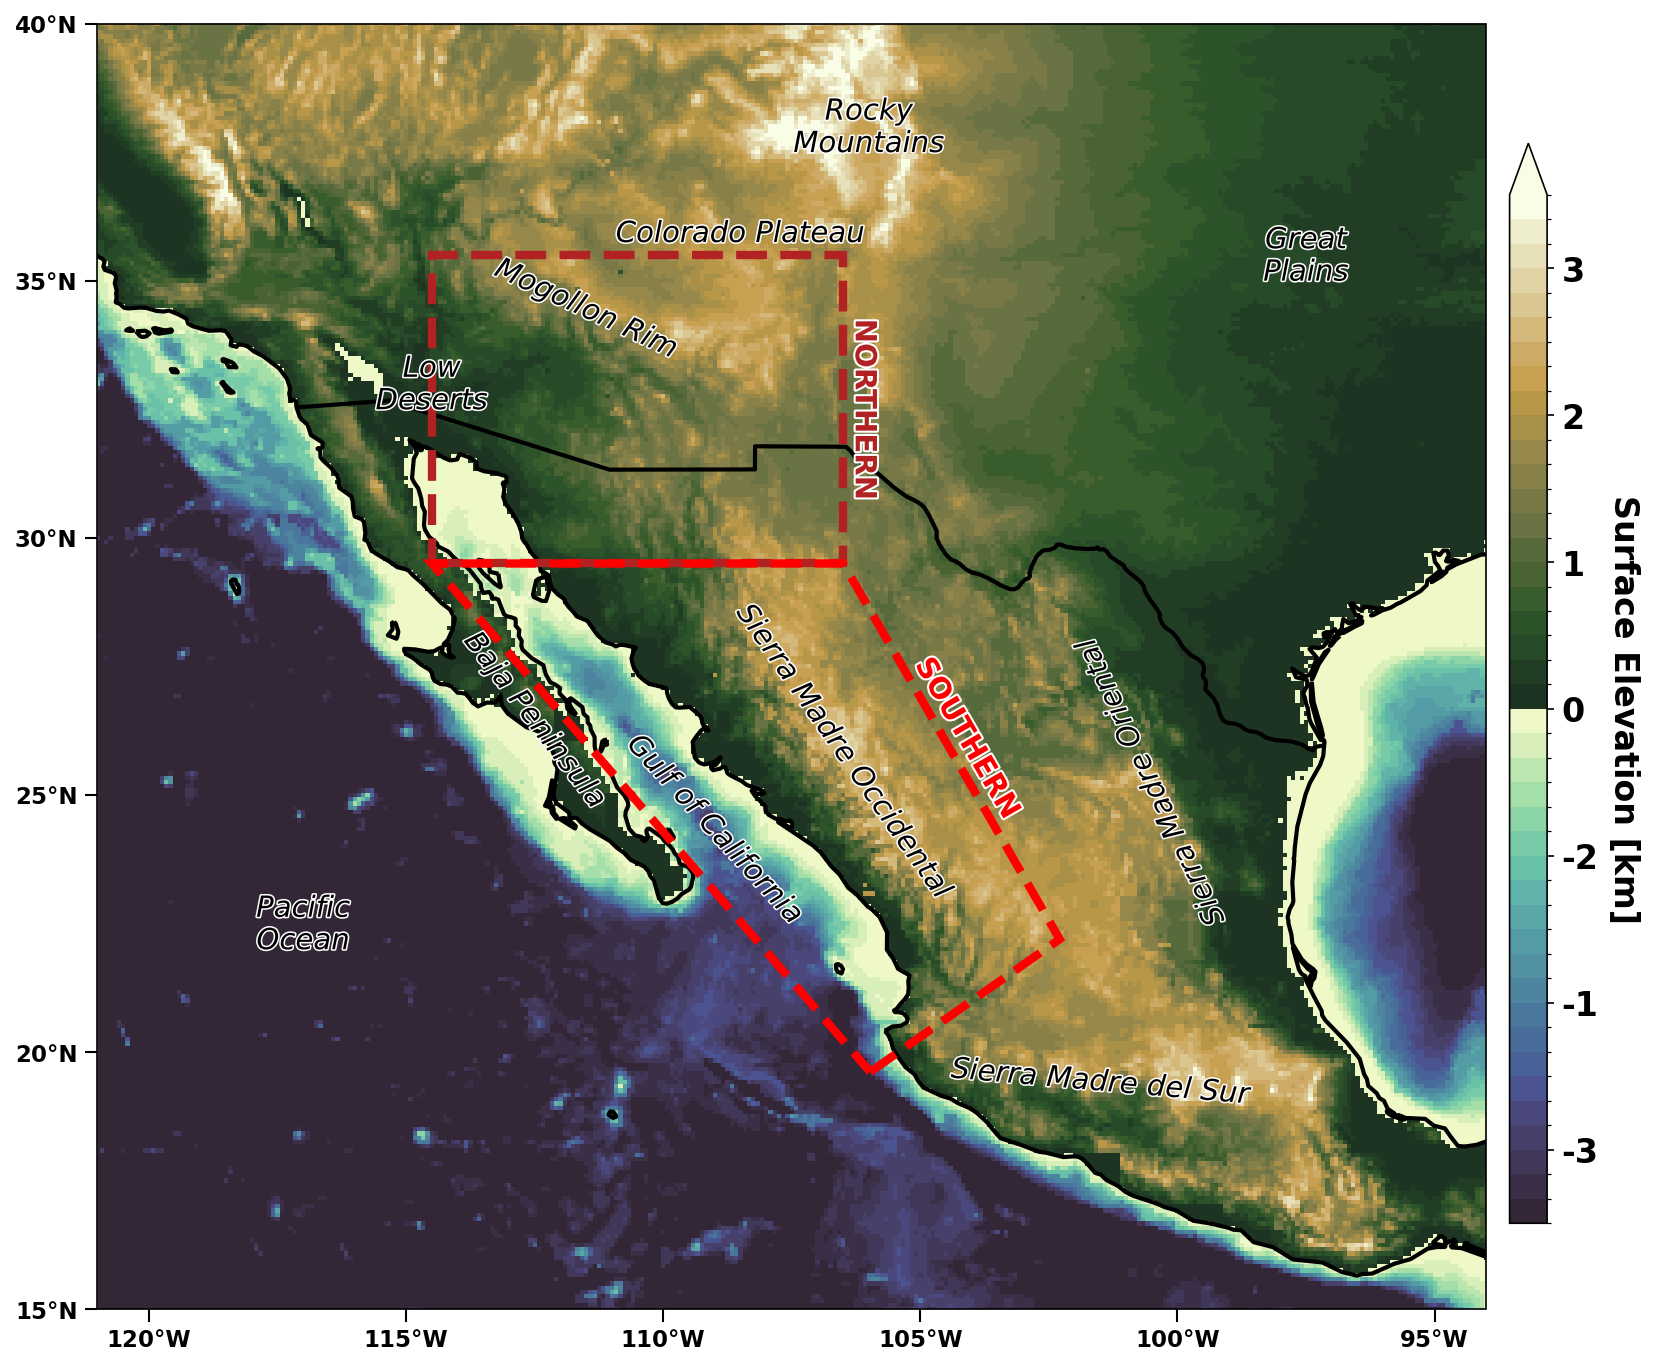
\includegraphics[width=\textwidth]{figs/fig_S1_study_region_geographic_features.png}\\
    \caption{Key physiographic features of the broader southwestern North America study region overlain on ETOPO05 topography and bathymetry. Dashed boxes outline limits of the Southern (light red) and Northern (dark red) Domains of the NAM region.}
    \label{fig:study-region}
\end{figure}

\begin{figure}[ht]
    \centering
    \includegraphics[width=
    \textwidth]{figs/fig_S1_prec_hrmip_historical_all_imerg_biases_maps.pdf}\\
    \caption{\textbf{All HighResMIP historical Jul.--Sept. (JAS) precipitation biases.} Bias in mean JAS precipitation in HighResMIP historical (1950--2014) simulations relative to mean observed JAS precipitation for IMERG observations (2001--2018). Each column corresponds to a model family and each row corresponds to bins of model resolutions, where biases in the lowest-resolution ($\geq$ 1\textdegree{}) configurations are in the top row, high-resolution (1\textdegree{} $>n\geq$ 0.5\textdegree{}) configurations are in the middle row, and ultra-high-resolution ($<$ 0.5\textdegree{}) configurations are in the bottom row. Dashed boxes outline limits of the Southern (light red) and Northern (dark red) Domains.}
    \label{fig:supp_hrmip-hist-biases-imerg}
\end{figure}

\begin{figure}[ht]
    \centering
    %\includegraphics[width=\textwidth]{figs/fig_S3_prec_hrmip_historical_.pdf}\\
    \caption{\textbf{Robustness of low- and high-resolution HighResMIP multi-model ensemble mean biases across observed precipitation products.} Biases in the low- and high-resolution multi-model ensemble mean Jul.--Sept. precipitation for the HighResMIP historical (1950--2014) simulations relative to mean observed Jul.--Sept. precipitation for 4 observations-based precipitation products (IMERG, TRMM, GPCP, GPCC). Dashed boxes outline limits of the Southern (light red) and Northern (dark red) Domains.}
    \label{fig:supp_hrmip-hist-mme-biases-all}
\end{figure}

\begin{figure}[ht]
    \centering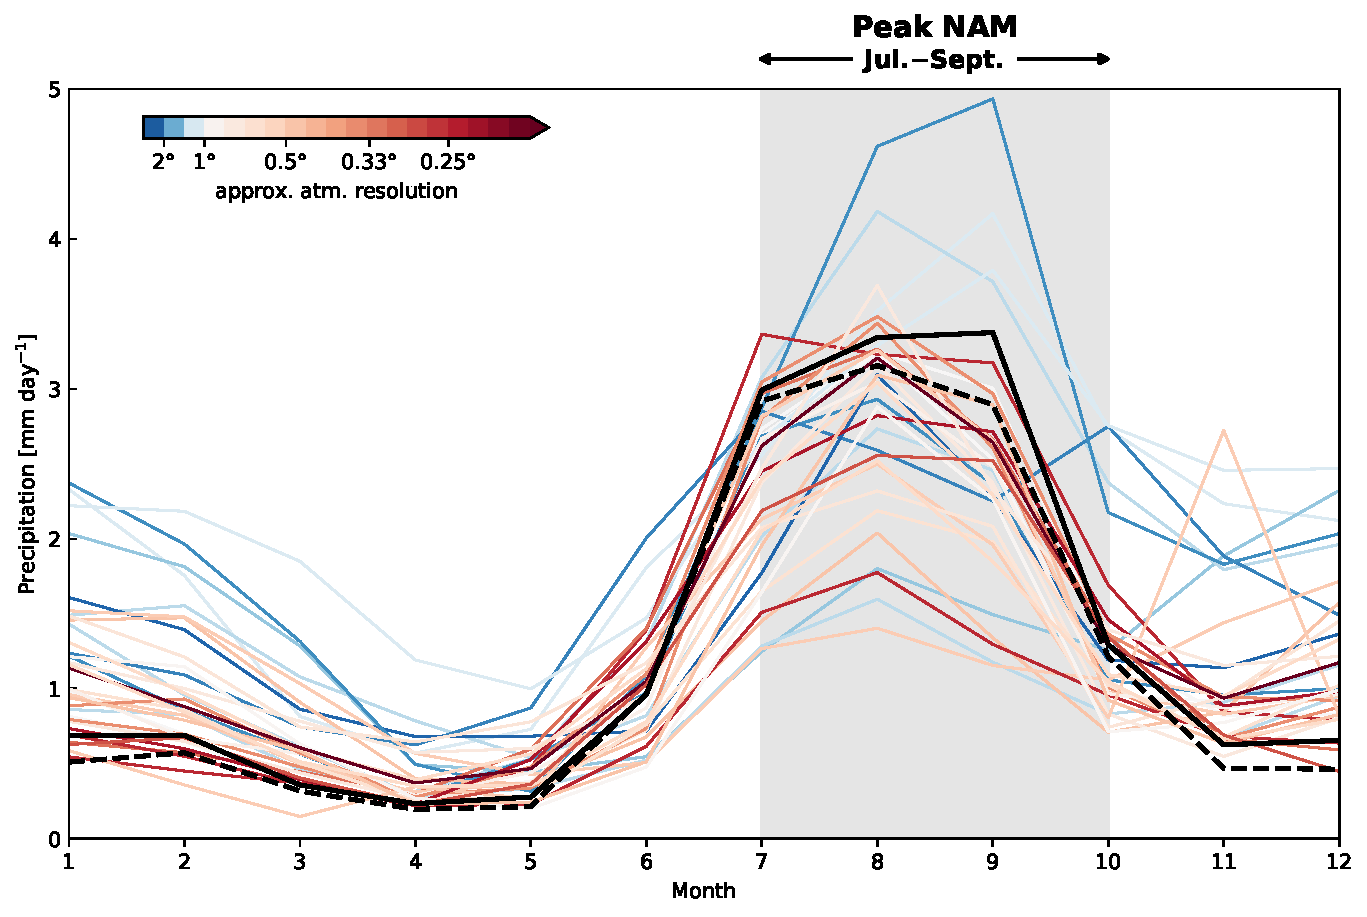
\includegraphics[width=\textwidth]{figs/fig_S4_prec_hrmip_historical_monthly_climo.pdf}
    \caption{\textbf{Monthly precipitation climatologies.} Mean annual cycle of precipitation averaged across the broader NAM region (20\textdegree{N}--35.5\textdegree{N}, 113\textdegree{W}--104\textdegree{W}) from monthly climatologies of IMERG (2001--2018; solid black line) and TRMM (1988--2013; dashed black line) observations compared to output from the HighResMIP models' historical experiments (1950--2014; colored lines). Line colors of HighResMIP climatologies correspond to the models' approximate horizontal resolution inferred from the length of the longitude coordinate. Grey shaded bar indicates timing of the peak NAM season.}
    \label{fig:supp_hrmip_hist_pr_climo}
\end{figure}

\begin{figure}[ht]
    \centering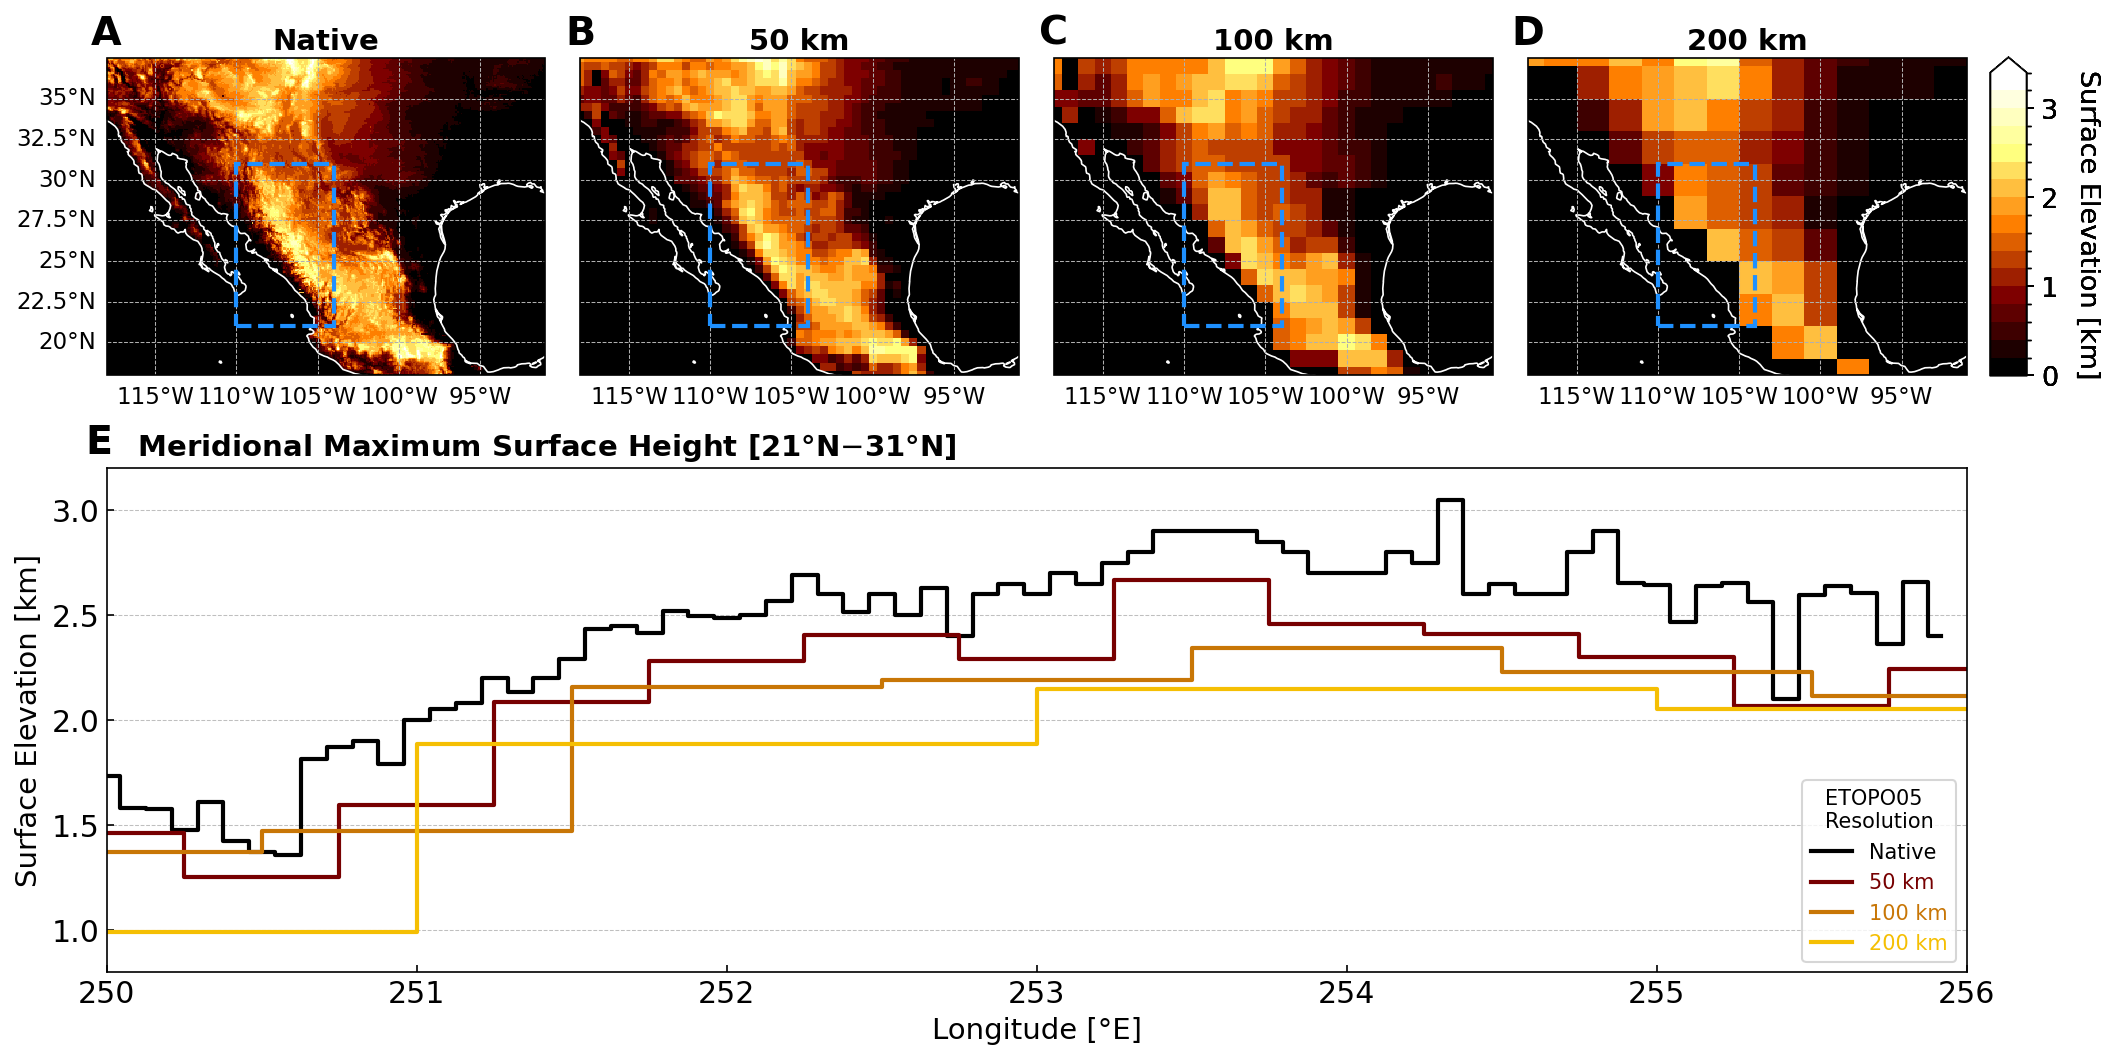
\includegraphics[width=\textwidth]{figs/fig_S5_topo_idealized_smo_profiles.png}
    \caption{\textbf{Reduction of Sierra Madre Occidental Peak heights with decreasing spatial resolution.} ETOPO05 observed elevation in northwest Mexico at (a) the product's native 5-minute resolution, or coarsened to a (b) 50 km, (c) 100 km, or (d) 200 km resolution. (e) Zonal profiles of meridional maximum surface height elevation within the dashed blue boxes on a--d (250\textdegree{E}--258\textdegree{E}, and 21\textdegree{N}--31\textdegree{N}), indicative of Sierra Madre Occidental peak heights.}
    \label{fig:etopo_idealized_regrid}
\end{figure}

\begin{figure}[ht]
    \centering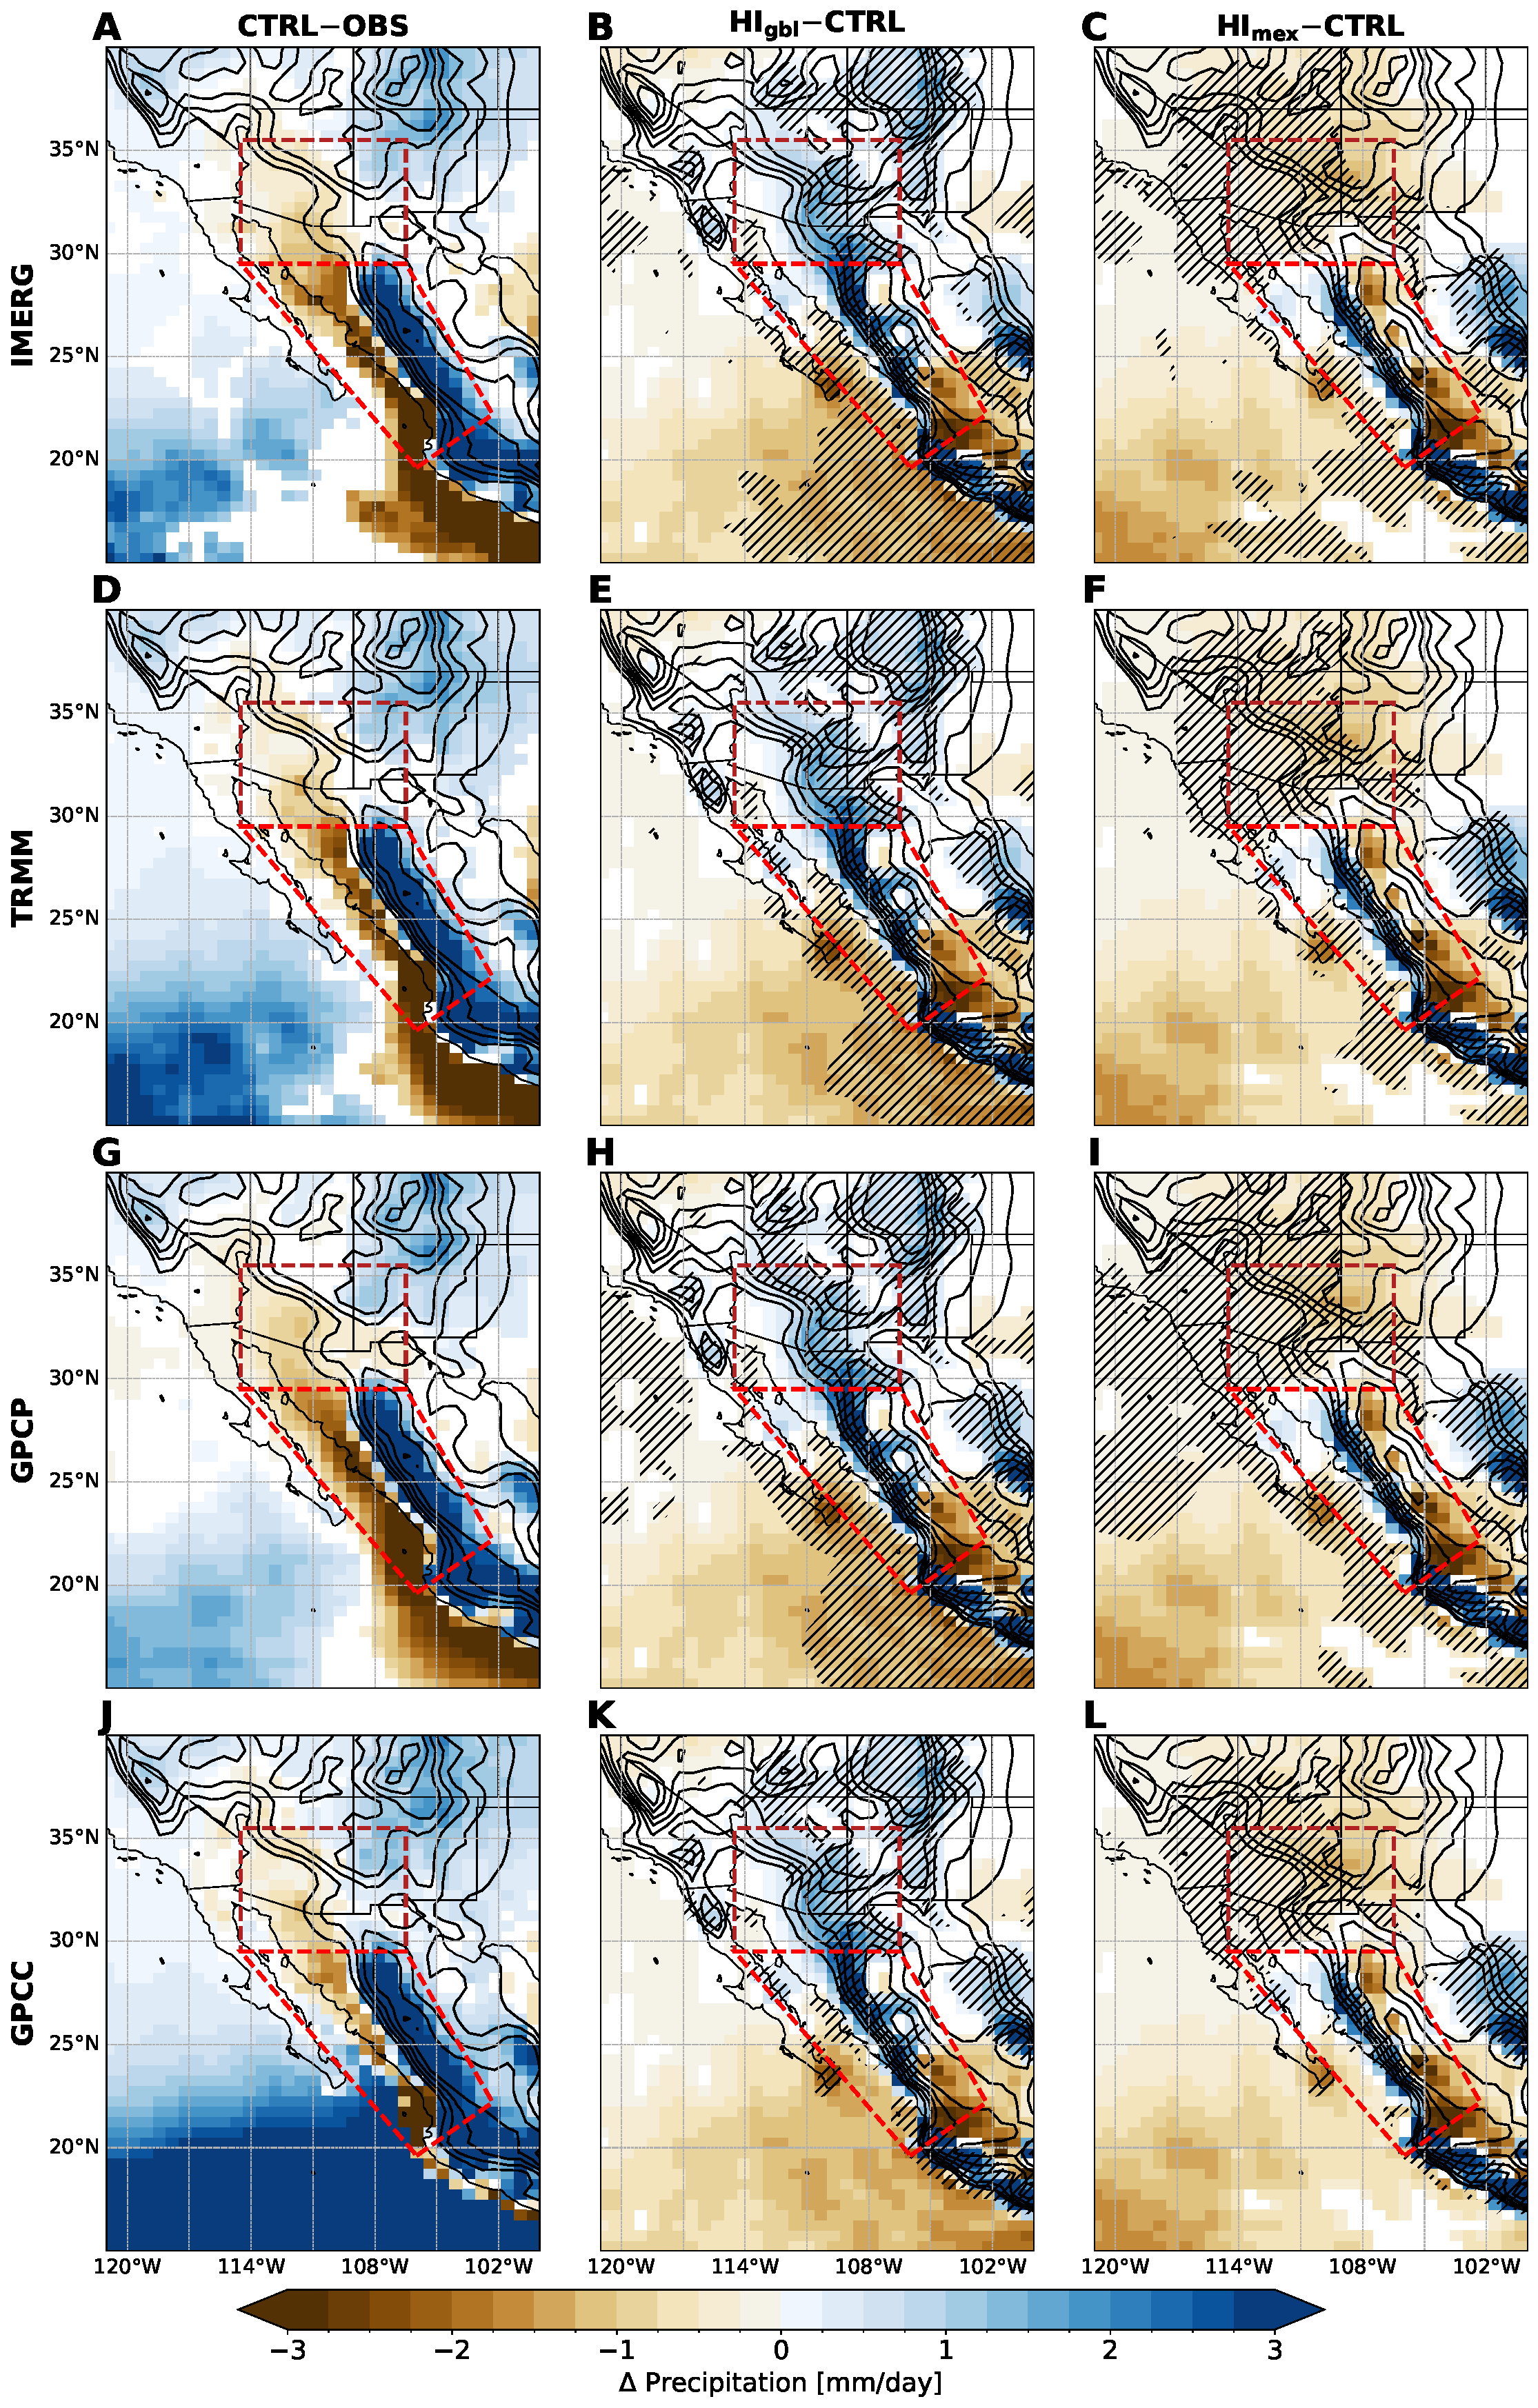
\includegraphics[width=.5\textwidth]{figs/fig_S6_prec_flor_pi_all-obs-prods-bias_change.pdf}
    \caption{\textbf{Impact of elevated topography on CM2.5-FLOR precipitation biases.} Biases in simulated Jul.--Sept. (JAS) precipitation in the preindustrial CM2.5-FLOR CTRL relative to observed precipitation products: (a) IMERG, (d) TRMM, (g) GPCP, and (j) GPCC \cite{rustemeir20gpcc}. Change in JAS simulated precipitation due to implementation of grid-cell maximum topography either (b,e,h,k) globally (HI$_{gbl}$), or (c,f,i,l) only over Mexico and Central America (HI$_{mex}$). The differences in simulated precipitation in the elevated topography sensitivity experiments plotted in the center and righthand columns are identical for each row, however, the hatching---which indicates where the change in precipitation due to elevated topography led to higher bias magnitudes than those in the CTRL simulation---does change given shifts in the absolute magnitude of the CTRL biases when compared to different observational precipitation products. Differences in precipitation are masked for statistical significance (p$<$0.1) based on two-sided Welch's t-test for panels (a,d,g,j) student's t-test for the remaining panels. Thin black contours outline model topography from 1 km to 4 km, intervals of 0.5 km. Dashed red boxes encompass the Northern (dark red) and Southern (light red) domains.}
    \label{fig:flor-biases-all-products}
\end{figure}

\begin{figure}[!htbp]
    \centering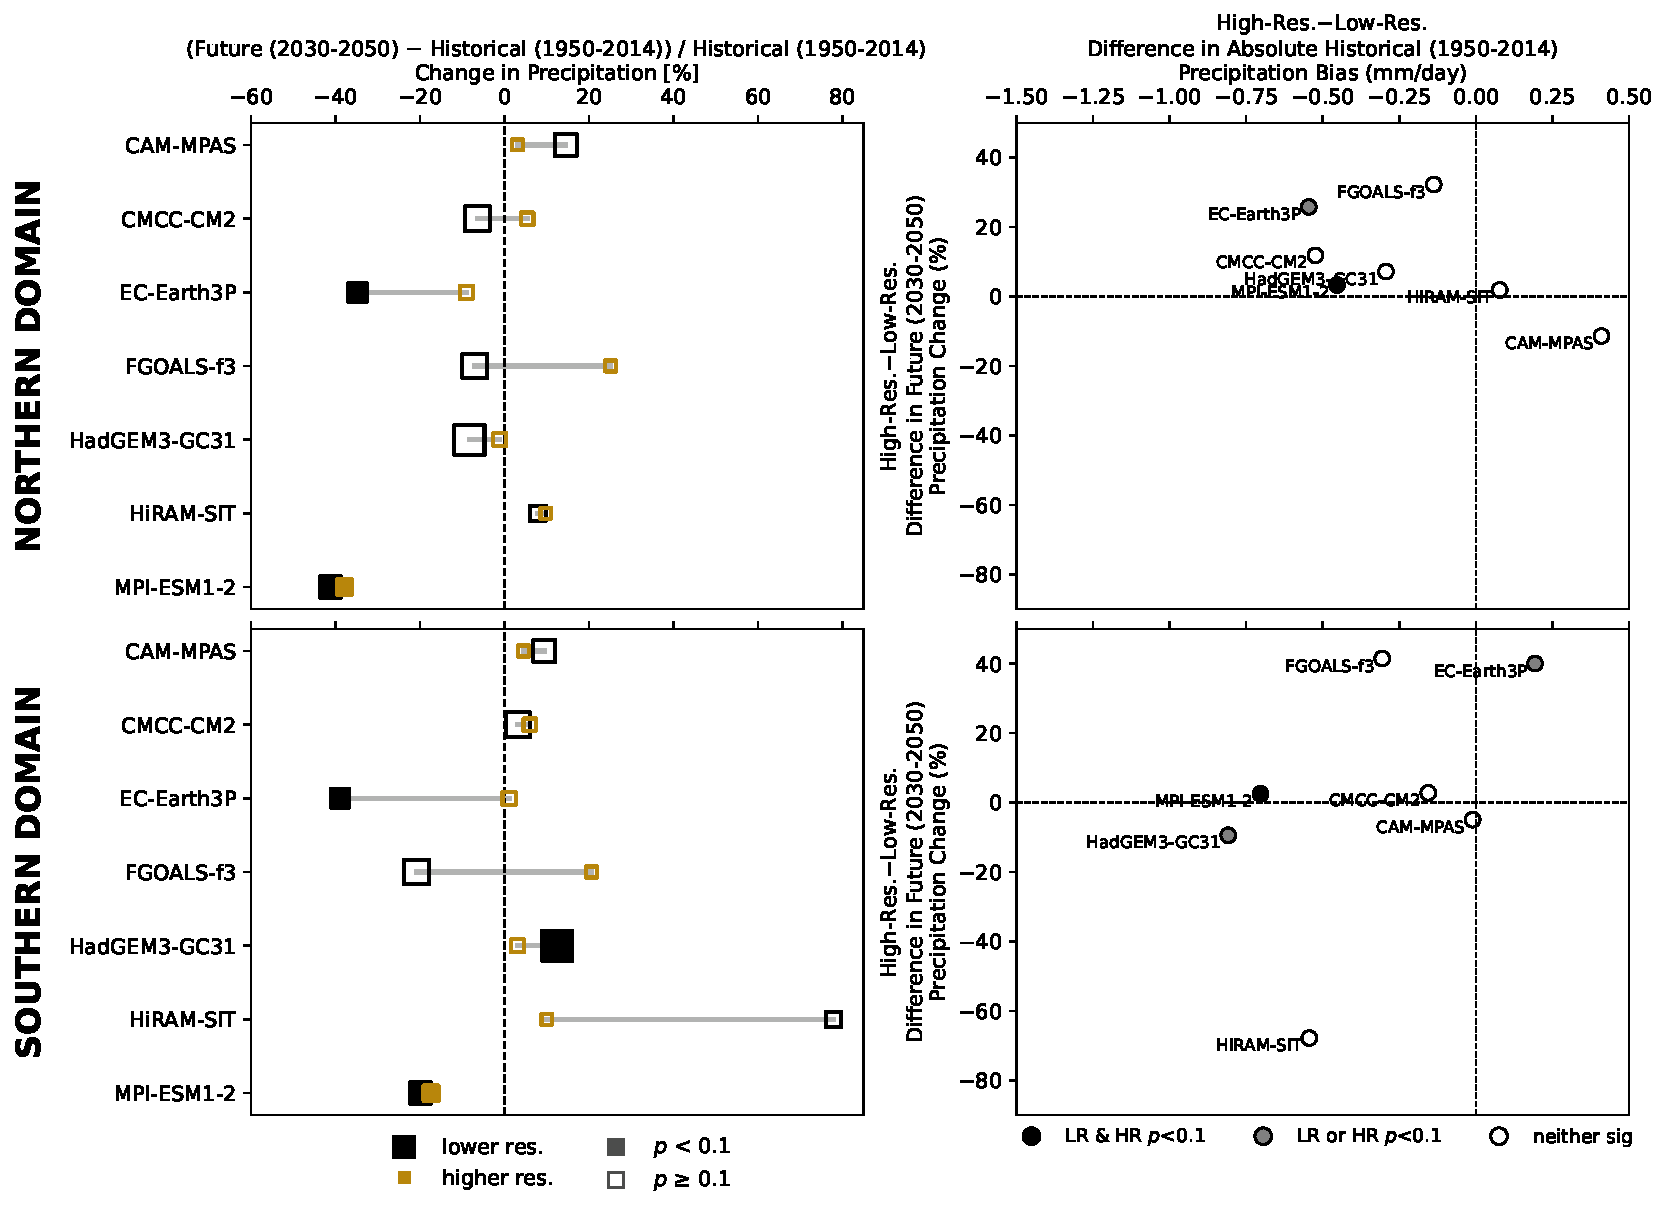
\includegraphics[width=\textwidth]{figs/fig_S7_prec_hrmip_future_delta_1950-2014_vs_2030-2050.pdf}
    \caption{\textbf{Impact of horizontal resolution on projected NAM rainfall in HighResMIP models.} Same as Figure 7, but compared to average rainfall during the full historical period (1950--2014).}
    \label{fig:future-prec-hrmip-2030}
\end{figure}

\begin{figure}[!htbp]
    \centering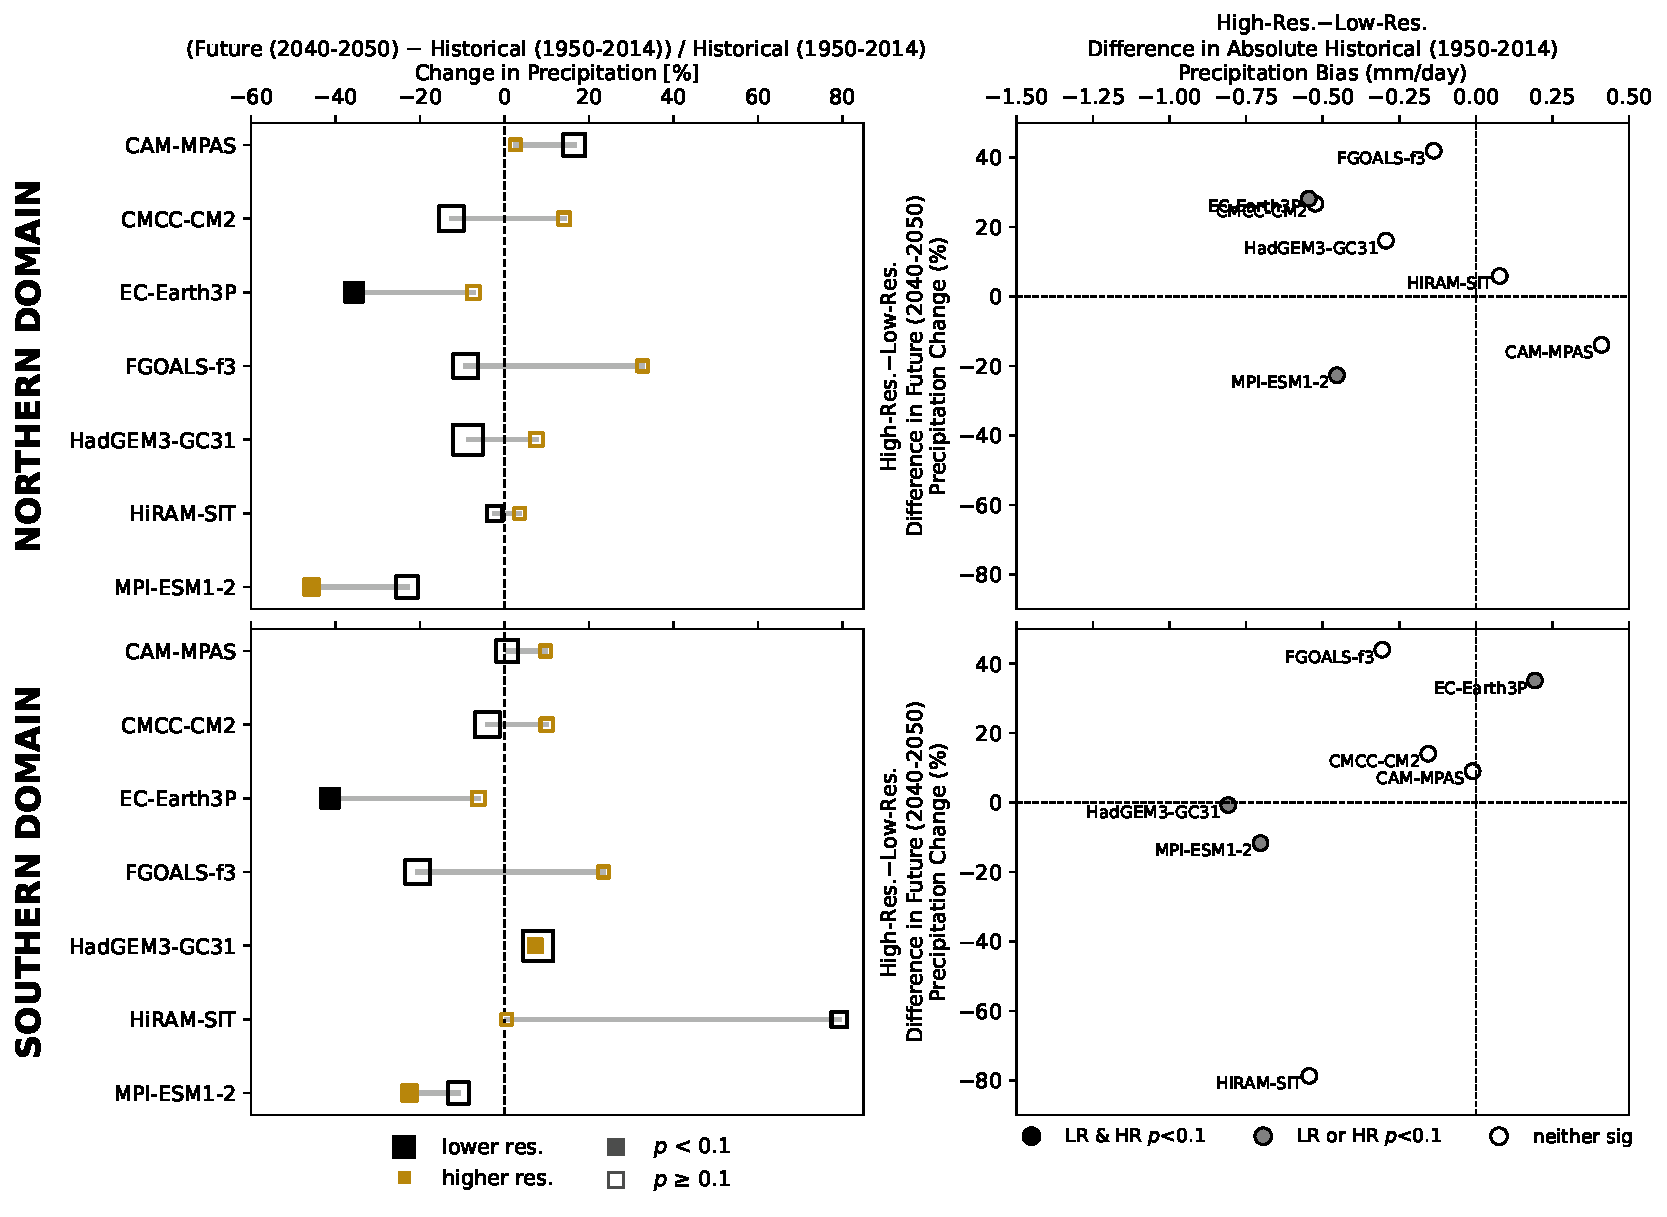
\includegraphics[width=\textwidth]{figs/fig_S8_prec_hrmip_future_delta_1950-2014_vs_2040-2050.pdf}
    \caption{\textbf{Impact of horizontal resolution on projected NAM rainfall in HighResMIP models.} Same as Figure 7, but for a shorter averaging period of mid-century projected rainfall (2040--2050) compared to average rainfall during the full historical period (1950--2014).}
    \label{fig:future-prec-hrmip-1979}
\end{figure}


%% ------------------------------------------------------------------------ %%
%%  TABLES

\begin{table}[htbp!]
\settablenum{S1}
\caption{HighResMIP \cite{haarsma16gmd} model details including their atmosphere component's grid-spacing and nominal resolution.}
\centering
\resizebox{\textwidth}{!}{
\begin{tabular}{ P{9cm} P{3cm} P{3.5cm} P{6cm} }
\toprule
\textbf{Institute} &
\textbf{Model} &
\makecell[l]{\textbf{Atm. Resolution}\\\textbf{lat$\times$lon (nominal)}} &
\textbf{Reference(s)} \\
\midrule

National Center for Atmospheric Research &
CAM-MPAS &
\makecell[l]{
180$\times$360 (100 km)\\
720$\times$1440 (25 km)} &
\citeA{sakaguchi23gmd} \\
\addlinespace[6pt]

Chinese Academy of Meteorological Sciences &
CAMS-CSM1-0 &
\makecell[l]{
160$\times$320 (100 km)\\
384$\times$768 (50 km)} &
\citeA{xin-yao19accr} \\
\addlinespace[6pt]

Centro Euro-Mediterraneo sui Cambiamenti Climatici &
CMCC-CM2 &
\makecell[l]{
192$\times$288 (100 km)\\
768$\times$1152 (25 km)} &
\citeA{cherchi19james} \\
\addlinespace[6pt]

Le Centre National de Recherches Météorologiques &
CNRM-CM6-1 &
\makecell[l]{
128$\times$256 (250 km)\\
360$\times$720 (50 km)} &
\citeA{voldoire19james} \\
\addlinespace[6pt]

EC-Earth Consortium &
EC-Earth3P &
\makecell[l]{
256$\times$512 (100 km)\\
512$\times$1024 (50 km)} &
\citeA{haarsma20gmdd} \\
\addlinespace[6pt]

European Centre for Medium-Range Weather Forecasts &
ECMWF-IFS &
\makecell[l]{
181$\times$360 (100 km)\\
361$\times$720 (50 km)} &
\citeA{roberts18gmd} \\
\addlinespace[6pt]

Chinese Academy of Sciences &
FGOALS-f3 &
\makecell[l]{
180$\times$288 (100 km)\\
720$\times$1440 (25 km)} &
\citeA{qing20aosl} \\
\addlinespace[6pt]

Geophysical Fluid Dynamics Laboratory &
GFDL-CM4 &
\makecell[l]{
180$\times$288 (100 km)\\
360$\times$576 (50 km)} &
\citeA{held19james} \\
\addlinespace[6pt]

Met Office Hadley Centre &
HadGEM3-GC31 &
\makecell[l]{
144$\times$192 (200 km)\\
324$\times$432 (100 km)\\
768$\times$1024 (50 km)} &
\citeA{roberts19gmd} \\
\addlinespace[6pt]

Research Center for Environmental Changes, Academia Sinica &
HiRAM-SIT &
\makecell[l]{
384$\times$768 (50 km)\\
768$\times$1536 (25 km)} &
\citeA{zhao09jc} \\
\addlinespace[6pt]

Institute for Numerical Mathematics &
INM-CM5 &
\makecell[l]{
120$\times$180 (250 km)\\
360$\times$540 (100 km)} &
\citeA{volodin17cd} \\
\addlinespace[6pt]

Institut Pierre Simon Laplace &
IPSL-CM6A &
\makecell[l]{
143$\times$144 (250 km)\\
361$\times$512 (100 km)} &
\citeA{boucher20james} \\
\addlinespace[6pt]

Max Planck Institute for Meteorology &
MPI-ESM1-2 &
\makecell[l]{
96$\times$192 (200 km)\\
192$\times$384 (100 km)\\
384$\times$768 (50 km)} &
\citeA{gutjahr19gmd} \\
\addlinespace[6pt]

Meteorological Research Institute &
MRI-AGCM3-2 &
\makecell[l]{
160$\times$320 (100 km)\\
320$\times$640 (50 km)\\
960$\times$1920 (25 km)} &
\citeA{mizuta12qi}, \citeA{kusunoki17a}\\

Japan Agency for Marine-Earth Science and Technology &
NICAM &
\makecell[l]{
320$\times$640 (100 km)\\
640$\times$1280 (25 km)} &
\citeA{kodama20gmdd} \\
\addlinespace[6pt]

\bottomrule
\end{tabular}}
\label{tab:S1-highresmip}
\end{table}


\end{document}